\section{Bil} \label{sec:bil}

\subsection{Klassediagram}
I dette afsnit beskrives det overordnede design på den software der kommer til at ligge på Pi. På figur \ref{fig:cd_pi} ses et klassediagram der opdeler funktionaliteten i klasser.

\begin{figure}[h]
\centering
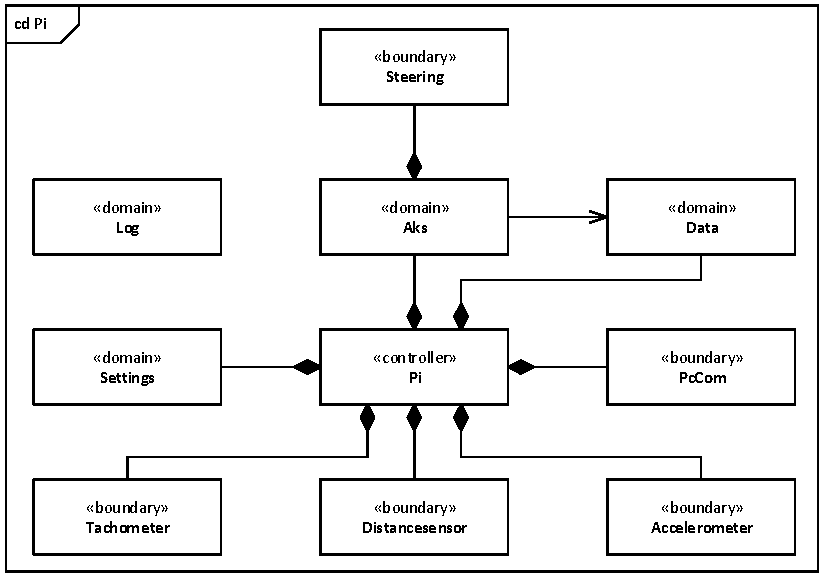
\includegraphics[width=\textwidth* 9/10]{../fig/diagrammer/bil/cd_pi.pdf}
\caption{Klasse diagram over Pi}
\label{fig:cd_pi}
\end{figure}

\subsubsection{Controller-klasse: Pi}
Controller-klassen Pi indeholder main funktionen og har derfor ansvaret for at styre slagets gang. Klassen skal derfor iværksætte initialisering af alle de klasser som den har ejerskab over. En af klassen ansvarsområder er at indsamle data fra sensorerne, og dette gøres ved at starte en særskilt tråd til dette. Denne tråd skal også sørge for at iværksætte Aks-klassen hver gang nye data er indsamlet.

\subsubsection{Domain-klasse: Aks}
Domain-klassen analyserer indkomne sensordata og i tilfælde at bilen er ved at køre ind i en forhindring, blokeres brugerinput og der styres udenom eller bremses.

\subsubsection{Domain-klasse: Data}
Denne klasse har til formål at indsamle alle sensordata i en datastruktur. Disse data gemmes i memory kan ikke overstige en defineret størrelse. Brugerinput gemmes ikke i denne klasse.

\subsubsection{Domain-klasse: Log}
Denne klasse har til formål at gemme samtlige systemhændelser i den fil, så kilden til eventuelle programcrash kan identificeres. Alle klasser på Pi har en reference til denne log, så de hver i sær kan skrive til den. På figur \ref{fig:cd_pi} er der undladt at lave pile fra alle klasser til denne, da dette vil gøre diagrammet uoverskueligt. 

\subsubsection{Domain-klasse: Settings}
Settings er datastruktur der indeholder indstillinger for maksimal hastighed, AKS status, og styretøjs kalibrering. Indstillingerne er gemt i en fil som kan tilgås af Pi-klassen og Steering-klassen.

\subsubsection{Boundary-klasse: PcCom}
Boundary-klassen PcCom håndterer kommunikationen imellem PC og Bil. Denne kommunikation sker vha. UDP via Wi-Fi.

\subsubsection{Boundary-klasse: Steering}
I denne klasse styres bilens aktautorer. Dette er altså en driver til både motoren der skaber fremdrift og servo-motoren der styrer forhjulene. Klassen tager ligeledes højde for brugers indstillinger.

\subsubsection{Boundary-klasse: Tachometer}
Denne klasse håndterer kommunikationen til bilens tachometer og konverterer sensordata til brugbar hastighedsmåling.

\subsubsection{Boundary-klasse: DistanceSensor}
Denne klasse håndterer kommunikationen til bilens afstandssensorer og konverterer sensordata til brugbar distancemålinger. Klasen håndterer alle fire sensorer.

\subsubsection{Boundary-klasse: Accelerometer}
Denne klasse håndterer kommunikationen til bilens accelerometer og konverterer sensordata til brugbar g-måling.

\clearpage

\subsection{Sekvensdiagrammer}
Herunder er udarbejdet sekvensdiagrammer for den funktionalitet som Pi blokken på bilen skal have. Der er tage udgangspunkt i de de tidligere fremstillede use cases. Sekvensdiagrammer for UC8 og UC12 er udeladt, da disse kun indeholder handlinger over interaktion imellem bruger og PC.

\begin{figure}[h]
\centering
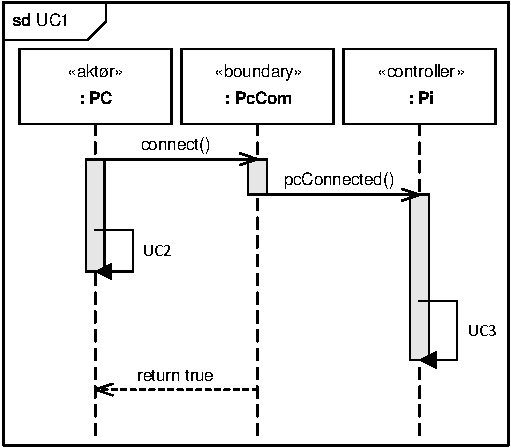
\includegraphics[]{../fig/diagrammer/bil/sd_uc1.pdf}
\caption{Sekvensdiagram over  bilens funktionalitet i UC1: Aktiver system}
\label{fig:sd_uc1_bil}
\end{figure}

\begin{figure}[h]
\centering
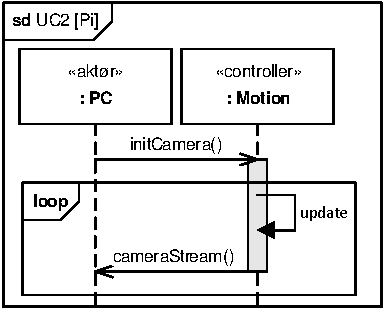
\includegraphics[]{../fig/diagrammer/bil/sd_uc2.pdf}
\caption{Sekvensdiagram over  bilens funktionalitet i UC2: Stream video}
\label{fig:sd_uc2_bil}
\end{figure}

\begin{landscape}

\begin{figure}[h]
\centering
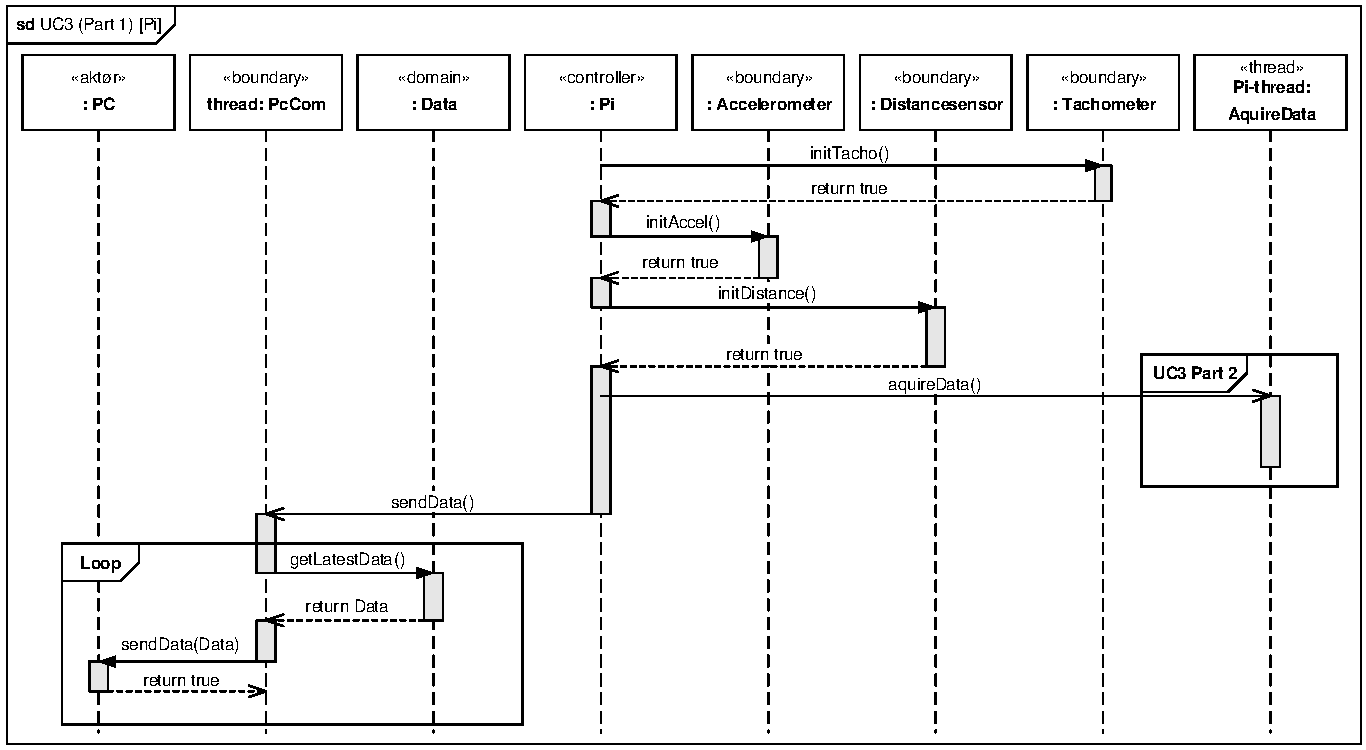
\includegraphics[]{../fig/diagrammer/bil/sd_uc3_1.pdf}
\caption{Sekvensdiagram over  bilens funktionalitet i UC3: Overvåg sensorer - Del 1}
\label{fig:sd_uc3_1_bil}
\end{figure}

\begin{figure}[h]
\centering
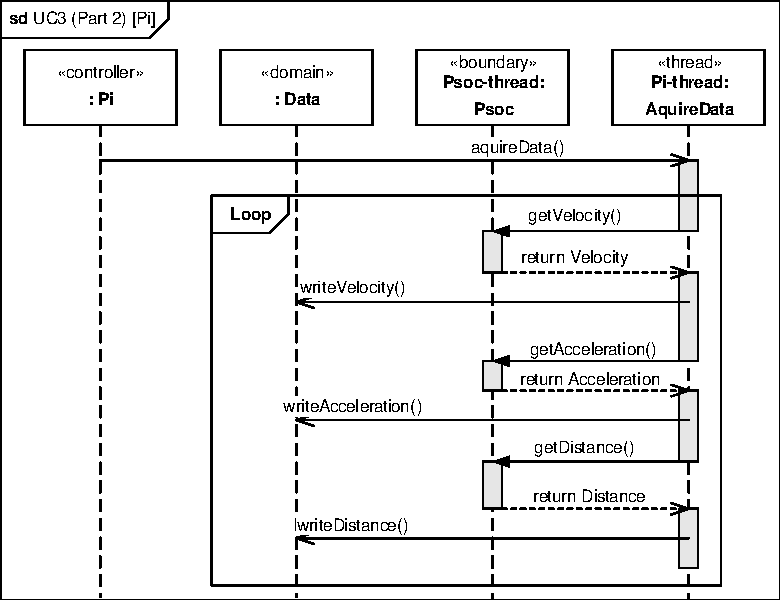
\includegraphics[]{../fig/diagrammer/bil/sd_uc3_2.pdf}
\caption{Sekvensdiagram over  bilens funktionalitet i UC3: Overvåg sensorer - Del 2}
\label{fig:sd_uc3_2_bil}
\end{figure}

\end{landscape}

\begin{figure}[h]
\centering
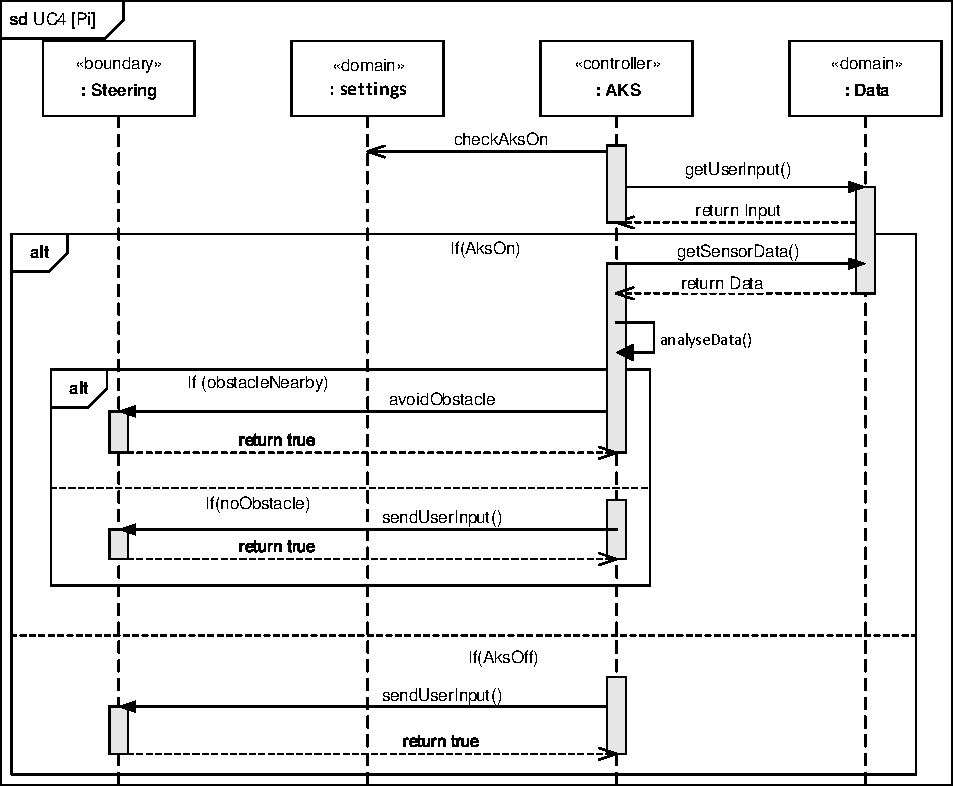
\includegraphics[]{../fig/diagrammer/bil/sd_uc4.pdf}
\caption{Sekvensdiagram over  bilens funktionalitet i UC4: Undvig forhindring}
\label{fig:sd_uc4_bil}
\end{figure}

\begin{figure}[h]
\centering
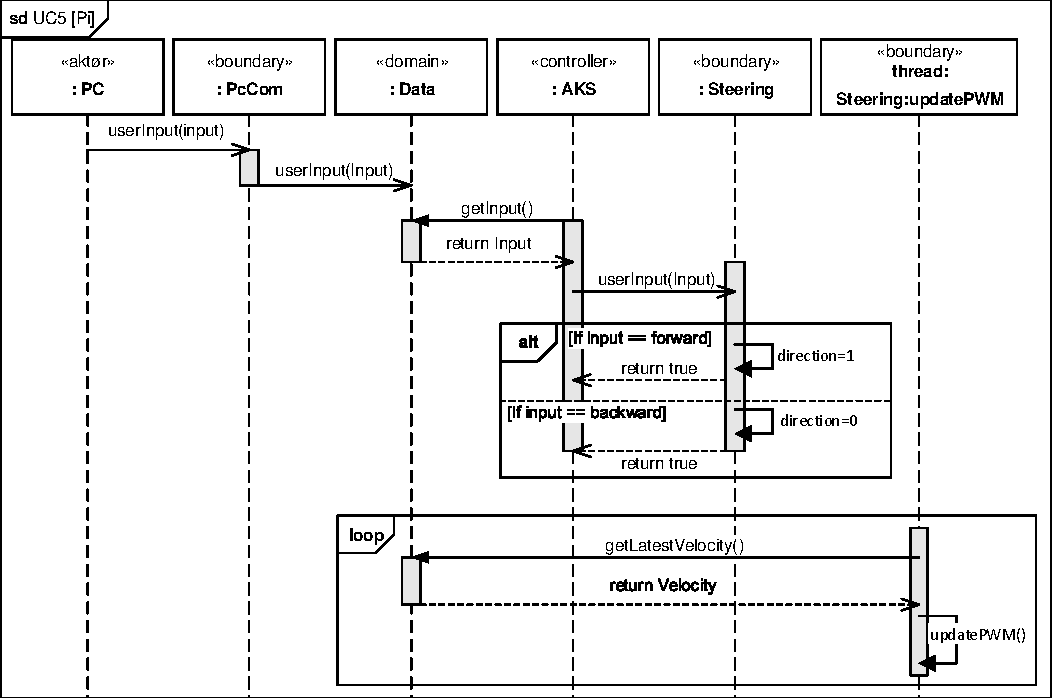
\includegraphics[]{../fig/diagrammer/bil/sd_uc5.pdf}
\caption{Sekvensdiagram over  bilens funktionalitet i UC5: Kør bil frem/tilbage}
\label{fig:sd_uc5_bil}
\end{figure}

\begin{figure}[h]
\centering
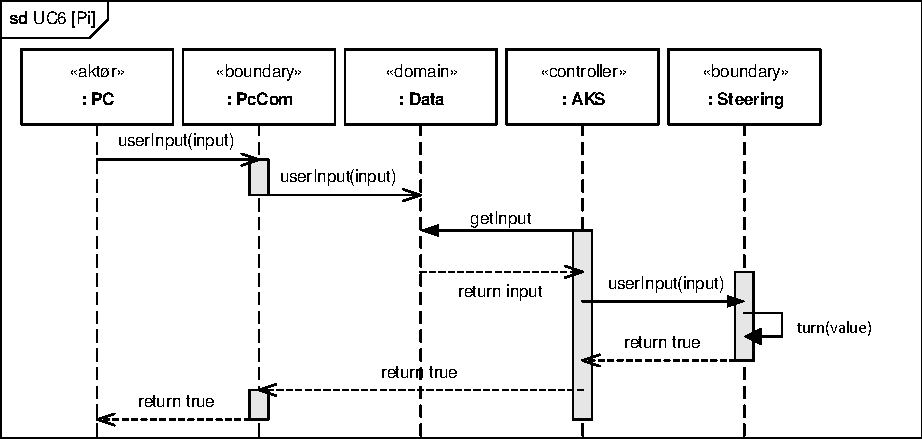
\includegraphics[]{../fig/diagrammer/bil/sd_uc6.pdf}
\caption{Sekvensdiagram over  bilens funktionalitet i UC6: Drej til højre/venstre}
\label{fig:sd_uc6_bil}
\end{figure}

\begin{figure}[h]
\centering
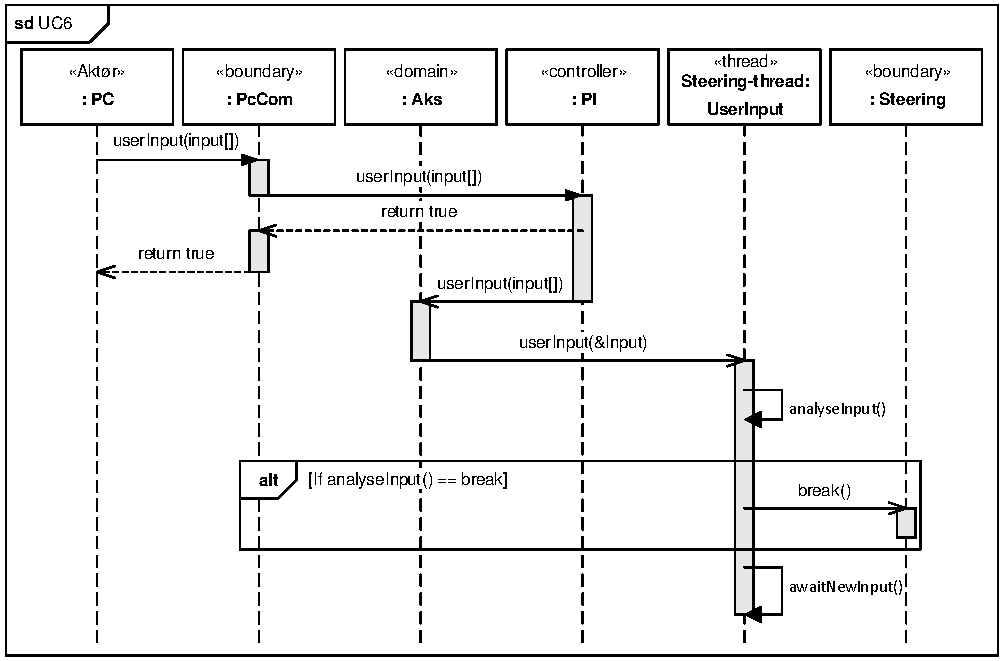
\includegraphics[]{../fig/diagrammer/bil/sd_uc7.pdf}
\caption{Sekvensdiagram over  bilens funktionalitet i UC7: Brems bil}
\label{fig:sd_uc7_bil}
\end{figure}

\begin{figure}[h]
\centering
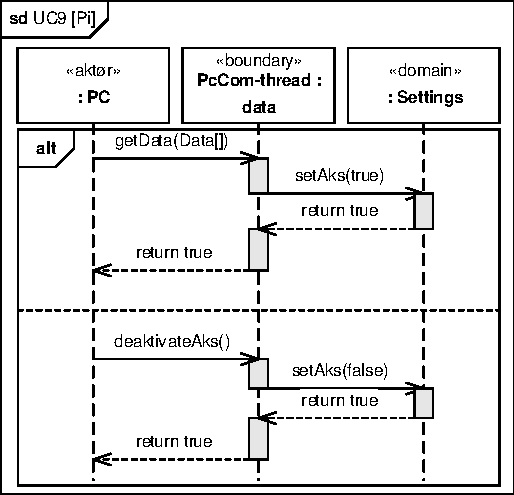
\includegraphics[]{../fig/diagrammer/bil/sd_uc9.pdf}
\caption{Sekvensdiagram over  bilens funktionalitet i UC9: Tænd/sluk AKS}
\label{fig:sd_uc9_bil}
\end{figure}

\begin{figure}[h]
\centering
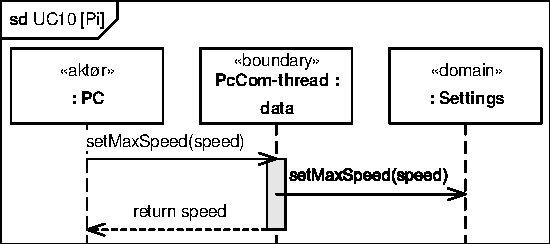
\includegraphics[]{../fig/diagrammer/bil/sd_uc10.pdf}
\caption{Sekvensdiagram over  bilens funktionalitet i UC10: Indstil makshastighed}
\label{fig:sd_uc10_bil}
\end{figure}

\begin{figure}[h]
\centering
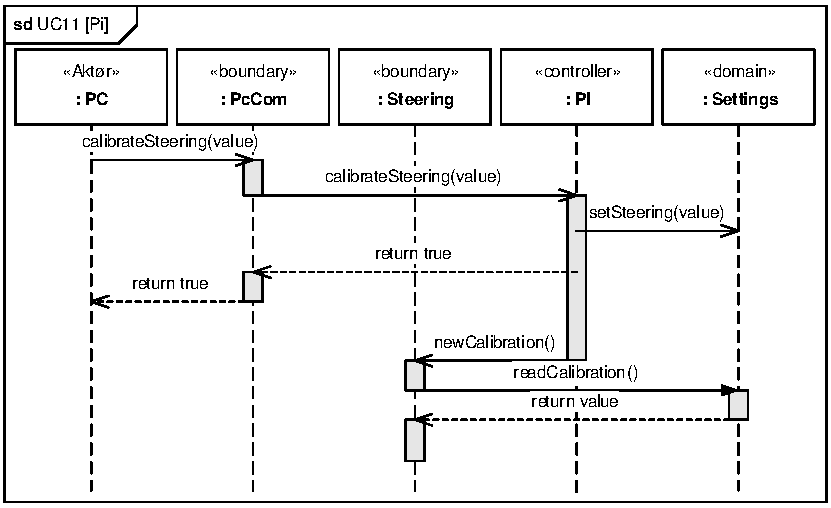
\includegraphics[]{../fig/diagrammer/bil/sd_uc11.pdf}
\caption{Sekvensdiagram over  bilens funktionalitet i UC11: Kalibrer styretøj}
\label{fig:sd_uc11_bil}
\end{figure}

\clearpage
\subsection{Klassebeskrivelser}
% ++++++++++++ Controller PSoC Master klassen ++++++++++++++
\subsubsection{Boundary-klasse: DistanceSensor}

Denne klasse har til formål at styre kommunikation mellem Pi og afstandssensorerne, der er valgt at benytte I2C-kommunikation til dette. De 4 afstandssensorer er navngivet efter deres respektive placering på bilen: ''Front Left'' = ''FL'', ''Front Left'' = ''FL'' ''Front Left'' = ''RL'', ''Rear Right'' = ''RR'', herefter funktion  \texttt{getDistance("name")} kaldes udefra med navnet på den ønskede sensor som parameter, og afstanden returneres i cm. Afstandene gemmes i midlertidige variabler. Desuden skrives der til den globale Log ved klasseinitiering og klassenedlæggelse, samt ved eventuelle forekomster af fejl.

\begin{figure}[h]
\centering
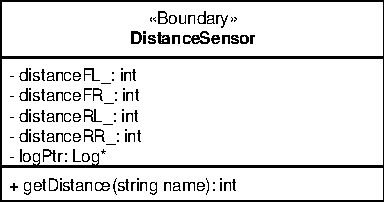
\includegraphics[]{../fig/diagrammer/bil/cd_distancesensor.pdf}
\caption{Klassebeskrivelse af boundary-klassen DistanceSensor}
\label{fig:cd_distancesensor}
\end{figure}

\textbf{Attributter}

\begin{table}[h]
	\begin{tabularx}{\textwidth}{| Z | Z | L{10cm} |} \hline
		Navn & Type & Beskrivelse \\\hline
		\texttt{distanceFL\_} & \texttt{int} 		& Midlertidig variabel der indeholder afstanden fra forreste venstre afstandssensor.\\\hline
		\texttt{distanceFR\_} & \texttt{int} 		& Midlertidig variabel der indeholder afstanden fra forreste højre afstandssensor.	\\\hline
		\texttt{distanceRL\_} & \texttt{int} 		& Midlertidig variabel der indeholder afstanden fra bagerste venstre afstandssensor \\\hline
		\texttt{distanceRR\_} & \texttt{int} 		& Midlertidig variabel der indeholder afstanden fra bagerste højre afstandssensor.	\\\hline
		\texttt{logPtr\_} 	 & \texttt{log*} 		& Pointer til at skrive i den globale Log											\\\hline
	\end{tabularx}
	\caption{Attributter for klassen DistanceSensor}
	\label{table:attr_distancesensor}
\end{table}
\clearpage

\textbf{Metoder}

\begin{table}[h]
	\begin{tabularx}{\textwidth}{| L{2.5 cm} | Z |} \hline
		Prototype 	& \texttt{int getDistance(string name)} \\\hline
		Parametre 	& \texttt{name} \newline Navnet på den sensor som der skal læses fra. Kan rumme én af fire muligheder "FL", "FR", "RL" og "RR". \\\hline
		Returværdi 	& \texttt{int} \newline Seneste afstandsmåling for den pågældende sensor. Værdien er angivet i cm. \\\hline
	\end{tabularx}
	\caption{Metodebeskrivelse for \texttt{getDistance}}
	\label{table:met_getdistance}
\end{table}
\clearpage